\section*{Introduction}

\M I was reflecting upon my notes, and realized how much I enjoyed
taking courses from Dr Albert Schwarz while at UC Davis. I also wanted
to review supermathematics, which I learned from Dr Schwarz during
Spring Quarter of 2008 in course Math 261B.

\M
We will study supermathematics by means of puzzles and exercises.
``Puzzles'' are more ``longterm'' questions to ponder, which we may
answer in future sections. ``Exercises'' are questions I want you to
answer as you read them. Or, if we think of this article as a road
trip, the ``puzzles'' are ``mileage signs'' and the ``exercises'' are the
next offramp.

\begin{figure}[h]
  \centering
  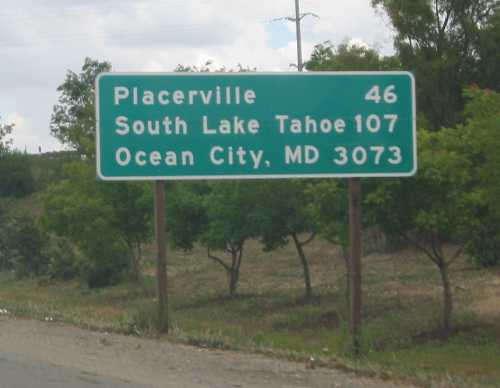
\includegraphics[width=7.55cm]{img/ocean-city.JPG}
  \caption[Mileage sign]{Every student at UC Davis recognizes this mileage sign on the
    Interstate-80 East. Note: 3073 miles is about 4945.5 kilometers. Taken from the DavisWiki, photo by Miriam Kaufman.\footnotemark}
\end{figure}
\footnotetext{See \url{https://localwiki.org/davis/Interstate_80} and \url{https://localwiki.org/davis/Interstate_80/_files/OceanCity.JPG/_info/}}

\section{Review of Algebras}

\M
Recall, an \define{Algebra} over a field $\FF$ consists of a vector
space $\mathcal{A}$ over $\FF$ equipped with a binary operator
$\cdot\colon\mathcal{A}\times\mathcal{A}\to\mathcal{A}$ called
\emph{multiplication} such that
\begin{enumerate}
\item Right distributivity: for any $a$, $b\in\FF$ and $v_{1}$, $v_{2}$, $w\in\mathcal{A}$,
  we have $(c_{1}v_{1}+c_{2}v_{2})\cdot w = c_{1}(v_{1}\cdot w) + c_{2}(v_{2}\cdot w)$.
\item Left distributivity: for any $a$, $b\in\FF$ and $v$, $w_{1}$, $w_{2}\in\mathcal{A}$,
  we have $v\cdot(c_{1}w_{1}+c_{2}w_{2}) = c_{1}(v\cdot w_{1}) + c_{2}(v\cdot w_{2})$.
\item Compatibility with scalar multiplication:
  for any $a$, $b\in\FF$ and $v$, $w\in\mathcal{A}$, we have
  $(av)\cdot(bw) = (ab)(v\cdot w)$.
\end{enumerate}
Authors often will call $\mathcal{A}$ an $\FF$-algebra. We do not
require multiplication in $\mathcal{A}$ to be associative (e.g., we
could take $\mathcal{A}=\RR^{3}$ and multiplication is the cross-product).

\begin{example}
  A grocery list of examples.
  \begin{enumerate}
  \item The complex numbers $\CC$ are an algebra over $\RR$
  \item The three-vectors in $\RR^{3}$ equipped with the usual
    cross-product form an algebra over $\RR$.
  \item The collection of polynomials with real coefficients form an
    algebra denoted $\RR[x]$, again over the field $\RR$.
  \item Let $n\in\NN$ be a fixed positive integer, let $\Mat(n,\FF)$
    denote the set of $n\times n$ matrices over $\FF$. Then it is a
    vector space when equipped with matrix addition and scalar
    multiplication is just multiplying componentwise by a scalar, and it
    is an algebra when equipped with matrix multiplication.
  \item We denote by $\gl(n,\FF)$ the vector space $\Mat(n,\FF)$
    equipped with multiplication given by $[X,Y]=XY-YX$ the commutator
    of matrices. This is a nonassociative algebra.
  \end{enumerate}
\end{example}

\N{Generating Set}
One way to express an algebra is to take a field $\FF$, then produce a
\define{Generating Set} $G$ which act as a basis for the free vector
space $\mathcal{A}=\FF\{G\}$ over $\FF$ (consisting of all [finite] linear combinations
$c_{1}g_{1}+\dots+c_{n}g_{n}$ where the $g_{i}\in G$ are distinct, and
$c_{i}\in\FF$) and demand the elements of $G$ [called the \define{Generators}
  of $\mathcal{A}$] satisfy some desired multiplication relations.

\begin{example}
  \begin{enumerate}
  \item The complex numbers have a single generator $\I$.
  \item The quaternions begin with $\FF=\RR$, then attach three generators $i$,
$j$, $k$ which satisfy $i^{4}=j^{4}=k^{4}=(ijk)^{2}=1$.
  \item The algebra $\RR^{3}$ equipped with the cross-product has three
    generators: $\vec{e}_{1}$, $\vec{e}_{2}$, and $\vec{e}_{3}$ (a.k.a.,
    the basis vectors) satisfying
    $\vec{e}_{i}\times\vec{e}_{j}=-\vec{e}_{j}\times \vec{e}_{i}$ for
    all $i,j=1,2,3$ and
    $\vec{e}_{1}\times\vec{e}_{2}=\vec{e}_{3}$,
    $\vec{e}_{3}\times\vec{e}_{1}=\vec{e}_{2}$, and
    $\vec{e}_{2}\times\vec{e}_{3}=\vec{e}_{1}$.
  \end{enumerate}
  This last example contains an important fact: it suffices to figure
  out the ``multiplication table'' for just the basis vectors (of the
  underlying vector space of $\mathcal{A}$). Specifically, how to write
  down
\begin{equation}
\vec{e}_{i}\vec{e}_{j} = \sum_{k=1}^{n}c_{i,j,k}\vec{e}_{k}
\end{equation}
where $c_{i,j,k}$ are scalars known as the \define{Structure Constants}.
\end{example}

\begin{definition}
We call the algebra $\mathcal{A}$ over $\FF$ \define{Unital} if there
exists an element $1\in\mathcal{A}$ such that for every
$x\in\mathcal{A}$ we have $x\cdot1=1\cdot x=x$.
\end{definition}
